	% Szglab4
% ===========================================================================
%
\chapter{Analízis modell kidolgozása 2}

\thispagestyle{fancy}

\section{Objektum katalógus}

\subsection{Robot}

A robotok azok az eszközök, amelyek a játék során versenyeznek egymással. Minden robotra egy felhasználó jut, aki irányíthatja azt. A robotok tudnak elhelyezni a pályán a olajfoltokat és ragacsfoltokat is. A robotok ugrással tudnak a cellákon keresztül a pályán haladni. Minden robotnak van sebessége és természetesen egy aktuális pozíciója is. A robotok tudják magukról, hogy mekkora távolságot tettek már meg a játék során, valamit azt is, hogy még hány olaj- illetve ragacsfolttal rendelkeznek. A robotok egymással ütközhetnek, aminek bekövetkeztekor erről szintén értesülhetnek.

\subsection{Cella}

A cellák tudják magukról, hogy olajfoltosak-e, ragacsfoltosak-e, vagy éppen üresek-e, - azaz egyik folt sem található meg rajtuk. A cellák összessége eredményezi a versenyzésre kijelölt pályát. A cella felelőssége az, hogy ha rálép egy mozgó objektum, akkor annak el tudja végezni a megfelelő utasításait, ilyen például a sebesség megfelezése, folt elhelyezése önmagán, vagy a robotok megsemmisítése.

\subsection{Pálya}

A pálya a cellák összességéből tevődik össze, amiben üres cellák is lesznek, azaz lyukak. Ezen a pályán versenyeznek a robotok valójában. A pálya tisztában van azzal, hogy hol van cella, s hol nincs. (Azaz, hogy melyik koordinátára ugorva marad életben a robot és melyik koordinátára ugorva hal meg.) A pálya tudja megadni az adott koordinátájú cella szomszédos, üresen álló celláit is. Erre akkor van szükség, ha két robot egyszerre szeretne ugyanarra a cellára ugrani. A pálya további felelőssége még, hogy a robotokat egymással összeütköztesse, ha esetleg azonos cellára lépnének. 

\subsection{Olajfolt}

A olajfoltok cellákon helyezkedhetnek el, illetve robotok tudják őket elhelyezni továbblépésük előtt, s ezek módosító hatással vannak az ezt követően belelépő robotokra: a robot sebessége nem lesz módosítható, a következő ugrás sebességvektora így ugyanakkora lesz, mint az előzőé.

\subsection{Ragacsfolt}

A ragacsfoltok szintén a cellákon helyezkedhetnek el, illetve a robotok tudják őket elhelyezni a továbblépésük előtt, s ezek módosító hatással vannak az ezt követően belelépő robotokra: megfelezik a robotok sebességének a nagyságát, tehát lassító hatással bírnak.


\clearpage
\section{Statikus struktúra diagramok}

\begin{figure}[!htbp]
\begin{center}
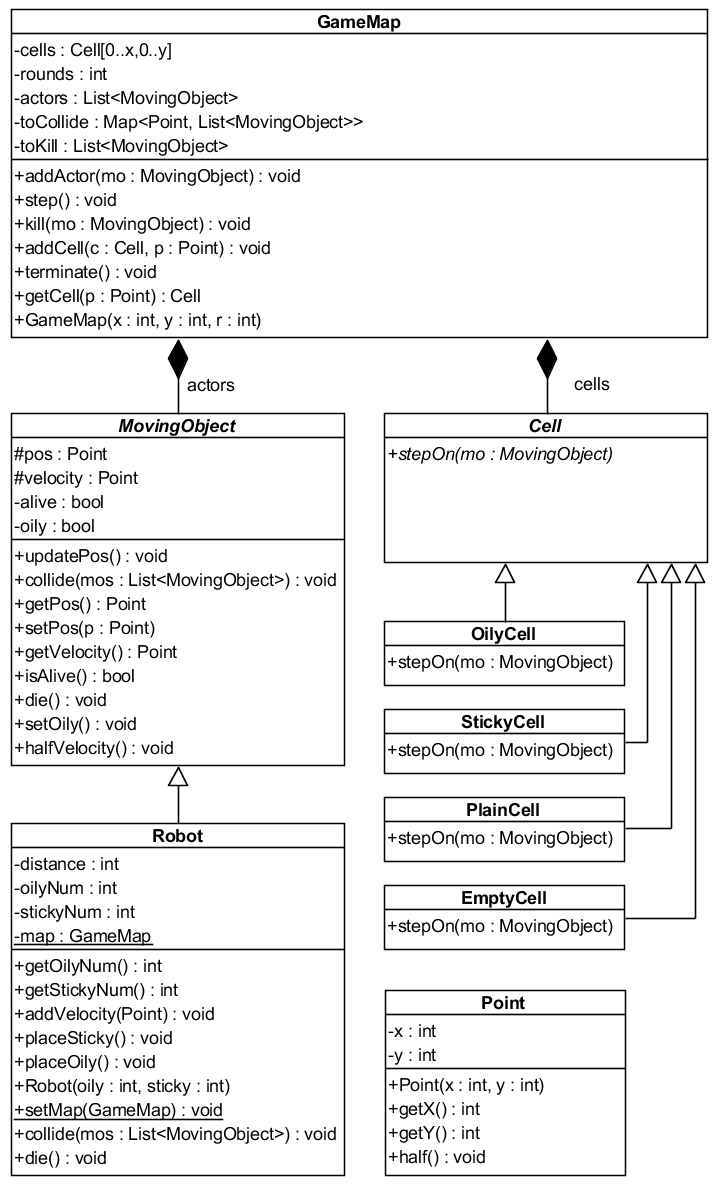
\includegraphics[width=13cm]{./chapters/chapter04/static.png}
\caption{A játék osztálydiagramja}
\end{center}
\end{figure}


\section{Osztályok leírása}
\subsection{Cell}
\begin{itemize}
	\item Felelősség\\
	Absztrakt osztály, a pálya egy celláját reprezentálja és alkalmazza a rálépő roboton az adott cellatípusra jellemző műveletet
	\item Metódusok
	\begin{itemize}
		\item void stepOn(MovingObject) : Absztrakt metódus, a paraméterként kapott objektumra alkalmazza a cellától elvárt műveletet.
	\end{itemize}
\end{itemize}

\subsection{EmptyCell}
\begin{itemize}
	\item Felelősség\\
	Az osztály felelőssége a pálya egy olyan cellájának reprezentációja, ami már nem képezi a robotok számára a pálya részét, azaz a rálépő robotok meghalnak.
	\item Ősosztályok\\
	MovingObject
	\item Metódusok
	\begin{itemize}
		\item void stepOn(MovingObject) : A paraméterként kapott objektumot utasítja, hogy ölje meg magát.
	\end{itemize}
\end{itemize}

\subsection{GameMap}
\begin{itemize}
\item Felelősség\\
Az osztály felelőssége a játék logikájához tartozó fő objektumok karbantartása és a játék léptetése. Ennek megfelelően rendelkezik az összes robottal, illetve a játék térképével. Ebből az osztályból minden játékhoz pontosan egy objektum tartozik.

\item Attribútumok
	\begin{itemize}
		\item cells: Cellákból álló mátrix, gyakorlatilag a térképet tárolja.
		\item rounds: A játékból hátralevő körök száma.
     	\item actors: A játékmenet belső aktorait, azaz a robotokat tárolja.
     	\item toCollide: Egy map adatstruktúra, ami a koordinátákkal indexelve tárolja, hogy az adott helyen melyik robotok állnak. A robotok ütköztetéséhez használjuk. Minden kör végén ürítjük.
     	\item toKill: Egy lista azokról a robotokról, amiket a kör végén meg kell ölni. Minden kör végén ürítjük.
	\end{itemize}
\item Metódusok
	\begin{itemize}
		\item void addActor(MovingObject) : Az actors listához hozzáadja a paraméterként kapott objektumot.
		\item void step() : A körök végén hívódik meg, a felelőssége a játék léptetése. Minden robotot utasít az ugrásra, ha leugrottak a pályáról akkor megöli őket, valamint utasítja az azokat a cellákat, amikre robotok ugrottak, hogy fejtsék ki hatásukat a rájuk ugró robotokra. Ezen kívül érzékeli ha egy cellán ütközés van és utasítja a robotokat a feloldására. Ha elfogytak a körök, leállítja a játékot.
		\item void kill(MovingObject) : Megöli a paraméterként kapott objektumot, azaz eltávolítja a játék logikájának nyilvántartásából (actors lista).
		\item void addCell(Cell, Point) : A térképen második paraméterként kapott helyre elhelyezi az első paraméterként kapott cellát.
		\item void terminate() : Leállítja a játékot és felszabadítja a már nem használt objektumokat.
		\item Cell getCell(Point) : A térképről visszaadja a paraméterként kapott pozíción álló cellát.
		\item GameMap(int x, int y, int r) : Az osztály konstruktora, létrehoz egy x*y méretű pályát, és beállítja a körök számát a harmadik paraméterként kapott r-re.
	\end{itemize}
\end{itemize}

\subsection{MovingObject}
\begin{itemize}
	\item Felelősség\\
	Egy absztrakt osztály, ami képes egy, a pályán mozgó objektumot reprezentálni, és elvégezni ennek a léptetését.
	\item Attribútumok
	\begin{itemize}
		\item pos : A mozgó objektum  pályán való elhelyezkedését tárolja.
		\item velocity : A mozgó objektum sebességét tárolja koordináták formájában.
		\item alive : Bool típusú változó, igaz ha a mozgó objektum életben van, hamis ha már meghalt (azaz kiesett a játékból).
		\item oily : Bool típusú változó, ha igaz az értéke, akkor az azt jelenti hogy a mozgó objektum olajos cellán áll, így a sebessége nem módosítható.
	\end{itemize}
	\item Metódusok
	\begin{itemize}
		\item void updatePos() : Lépteti a mozgó objektumot, azaz hozzáadja a helyzetéhez a sebességét (vektoriálisan).
		\item void collide(List<MovingObject>) : A paraméterként kapott listában szereplő mozgó objektumokat ütközteti egymással. (A listában önmagának is benne kell lennie.) Ha van a cella szomszédságában elegendő olyan cella amin nem áll robot, akkor mindegyik ütköző robotot áthelyezi egy ilyenre, különben megöli őket.
		\item Point getPos() : Visszaadja a mozgó objektum jelenlegi pozícióját a pályán.
		\item void setPos(Point) : A paraméterként kapott helyre helyezi a mozgó objektumot, azaz beállítja a pos változót.
		\item Point getVelocity() : Visszaadja a mozgó objektum aktuális sebességét.
		\item bool isAlive() : Igazzal tér vissza ha a mozgó objektum életben (játékban) van, különben hamissal.
		\item void die() : Megöli a mozgó objektumot.
		\item void setOily() : Beálltja az oily attribútum értékét igazra, azaz megtiltja a sebességvektor módosítását az adott körben.
		\item void halfVelocity() : Megfelezi a mozgó objektum sebességét, ragacsos cellánál használandó.
	\end{itemize}
\end{itemize}

\subsection{OilyCell}
\begin{itemize}
	\item Felelősség\\
	Az osztály felelőssége a pálya egy olajfoltos cellájának reprezentációja és a rálépő robot számára annak megtiltása, hogy a sebességét módosítsák.
	\item Ősosztályok\\
	MovingObject
	\item Metódusok
	\begin{itemize}
		\item void stepOn(MovingObject) : A paraméterként kapott objektumot utasítja, hogy tiltsa le a sebességvektor módosításának lehetőségét.
	\end{itemize}
\end{itemize}

\subsection{PlainCell}
\begin{itemize}
	\item Felelősség\\
	Az osztály felelőssége a pálya egy folt nélküli cellájának reprezentációja.
	\item Ősosztályok\\
	MovingObject
	\item Metódusok
	\begin{itemize}
		\item void stepOn(MovingObject) : Egy folt nélküli celláról lévén szó, nem tesz semmit a paraméterként kapott objektummal.
	\end{itemize}
\end{itemize}

\subsection{Point}
\begin{itemize}
	\item Felelősség\\
	Az osztály egy koordinátapárt képes tárolni, és ezen műveleteket végezni.
	\item Attribútumok
	\begin{itemize}
		\item x: A pont X koordinátája.
		\item y: A pont Y koordinátája.
	\end{itemize}
	\item Metódusok
	\begin{itemize}
		\item Point(int x, int y): Konstruktor, paraméterként a pont X és Y koordinátáit kapja meg és állítja be a megfelelő attribútumnak.
		\item int getX(): A tárolt pont X koordinátáját adja vissza.
		\item int getY(): A tárolt pont Y koordinátáját adja vissza.
		\item void half(): A tárolt pont mindkét koordinátáját a felére csökkenti (alsó egész részt véve).
	\end{itemize}
\end{itemize}

\subsection{Robot}
\begin{itemize}
	\item Felelősség\\
	Az osztály felelőssége egy robot reprezentációja, és a robot cselekedeteinek irányíthatóságának biztosítása kifele.
	\item Ősosztályok\\
	MovingObject
	\item Attribútumok
	\begin{itemize}
		\item distance : A robot által eddig megtett távolságot tárolja.
		\item oilyNum : A robot rendelkezésére álló olajos foltok számát tárolja.
		\item stickyNum : A robot rendelkezésére álló ragacsos foltok számát tárolja.
		\item map : Statikus attribútum, az adott játékmenethez biztosít hozzáférést.
	\end{itemize}
	\item Metódusok
	\begin{itemize}
		\item int getOilyNum() : Visszaadja a robot rendelkezésére álló olajos foltok számát.
		\item int getStickyNum() : Visszaadja a robot rendelkezésére álló ragacsos foltok számát.
		\item void addVelocity(Point) : A paraméterként kapott sebességvektorral megnöveli a robot jelenlegi sebességét.
		\item void placeSticky() : A robot a jelenlegi pozícióján elhelyez egy ragacsfoltot.
		\item void placeOily() : A robot a jelenlegi pozícióján elhelyez egy olajfoltot.
		\item Robot(int oily, int sticky) : Az osztály konstruktora, inicializálja a rendelkezésre álló foltok számát a paraméterek alapján, valamint 0-ra állítja a robot sebességét és az általa megtett távolságot. Ezen kívül élőre állítja a robot állapotát és engedélyezi a sebesség módosítását.
		\item void setMap(GameMap) : Beállítja a map attribútumot a paraméterként kapott értékre, azaz hozzáférést ad a robotnak az adott játékmenethez.
		\item void collide(List<MovingObject>) : A paraméterként kapott mozgó objektumokkal ütközteti a robotot a MovingObject osztályban leírt módon. Fontos, hogy paraméterként önmagát is megkapja.
		\item void die() : Megöli az adott robotot, azaz eltávolíttatja magát az aktuális játékmenetből.
	\end{itemize}
\end{itemize}

\subsection{StickyCell}
\begin{itemize}
	\item Felelősség\\
	Az osztály felelőssége a pálya egy ragacsfoltos cellájának reprezentációja és a rálépő robot sebességének megfelezése.
	\item Ősosztályok\\
	MovingObject
	\item Metódusok
	\begin{itemize}
		\item void stepOn(MovingObject) : A paraméterként kapott objektumot utasítja, hogy felezze meg a sebességét.
	\end{itemize}
\end{itemize}


\clearpage
\section{Szekvencia diagramok}


\begin{figure}[!htbp]
	\begin{center}
		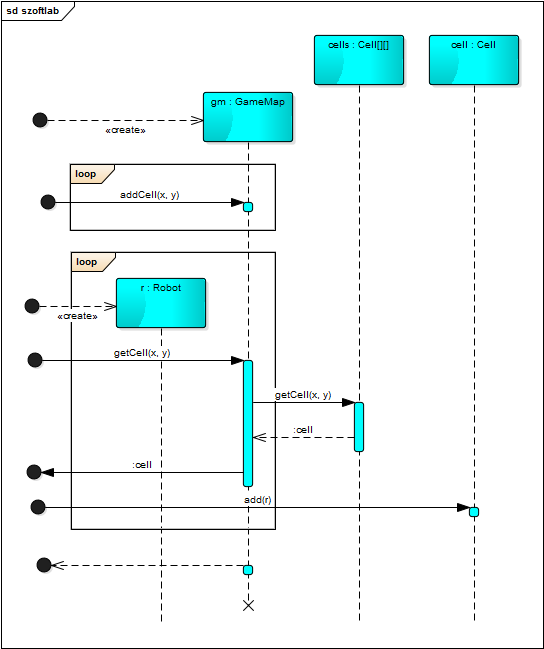
\includegraphics[width=166mm, center]{./vegleges_statikus_seq/GameMap.png}
		\caption{Játék indítása}
	\end{center}
\end{figure}

\begin{figure}[!htbp]
	\begin{center}
		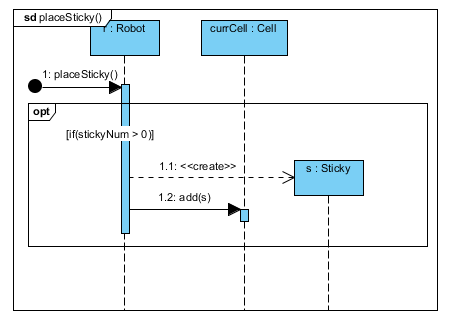
\includegraphics[width=166mm, center]{./vegleges_statikus_seq/placesticky.png}
		\caption{Olajfolt hátrahagyása}
	\end{center}
\end{figure}

\begin{figure}[!htbp]
	\begin{center}
		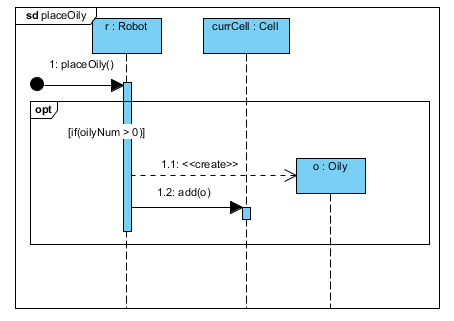
\includegraphics[width=166mm, center]{./vegleges_statikus_seq/placeoily.png}
		\caption{Ragacsfolt hátrahagyása}
	\end{center}
\end{figure}

\clearpage

\begin{figure}[!htbp]
	\begin{center}
		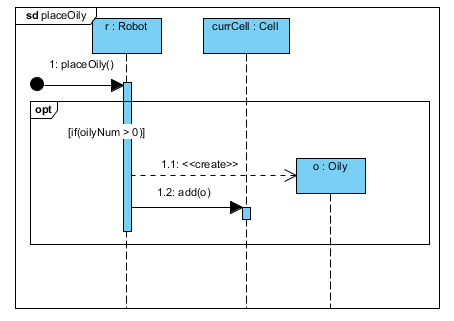
\includegraphics[width=166mm, center]{./vegleges_statikus_seq/placeoily.png}
		\caption{Ragacsfolt hátrahagyása}
	\end{center}
\end{figure}

%\begin{figure}[!htbp]
%	\begin{center}
%		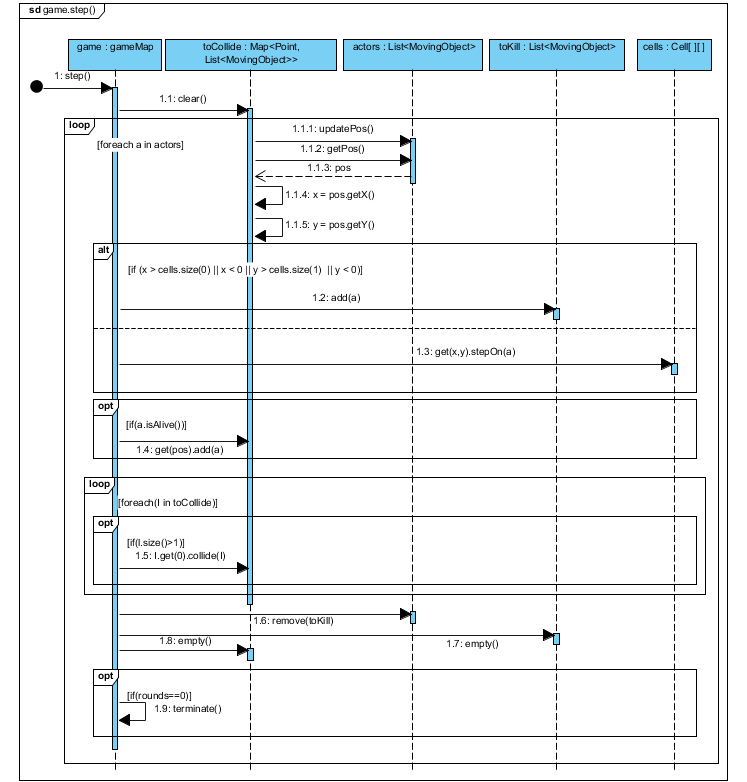
\includegraphics[width=195mm, center]{./chapters/chapter04/step.png}
%		\caption{A játék léptetése}
%	\end{center}
%\end{figure}

\begin{figure}[!htbp]
	\begin{center}
		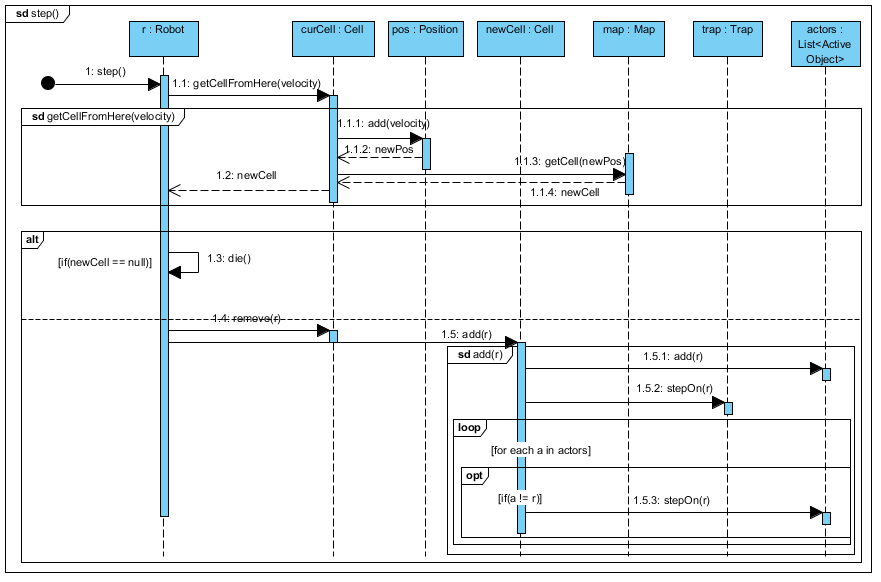
\includegraphics[width=166mm, center]{./vegleges_statikus_seq/step.png}
		\caption{A robot lép}
	\end{center}
\end{figure}

%\begin{figure}[!htbp]
%	\begin{center}
%		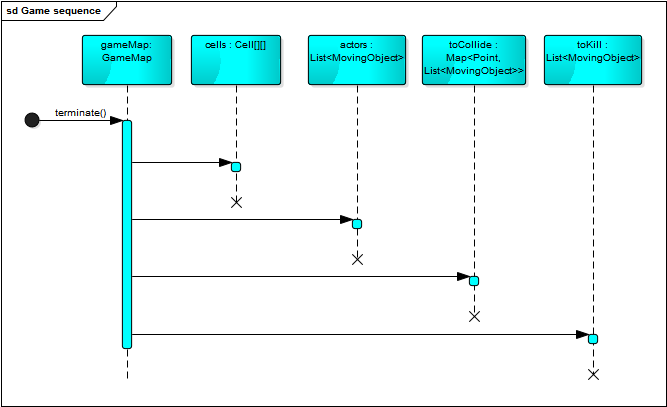
\includegraphics[width=180mm, center]{./chapters/chapter04/Gamesequence.png}
%		\caption{}
%	\end{center}
%\end{figure}

\begin{figure}[!htbp]
	\begin{center}
		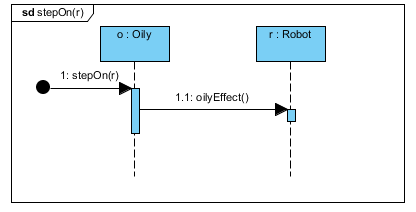
\includegraphics[width=166mm, center]{./vegleges_statikus_seq/steponoily.png}
		\caption{A robot olajba lép}
	\end{center}
\end{figure}

\begin{figure}[!htbp]
	\begin{center}
		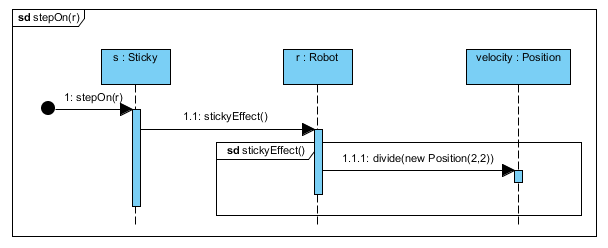
\includegraphics[width=166mm, center]{./vegleges_statikus_seq/steponsticky.png}
		\caption{A robot ragacsba lép}
	\end{center}
\end{figure}

\begin{figure}[!htbp]
	\begin{center}
		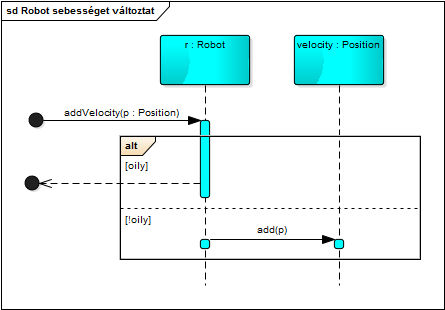
\includegraphics[width=166mm, center]{./vegleges_statikus_seq/changevelocity.png}
		\caption{A robot ragacsba lép}
	\end{center}
\end{figure}

\begin{figure}[!htbp]
	\begin{center}
		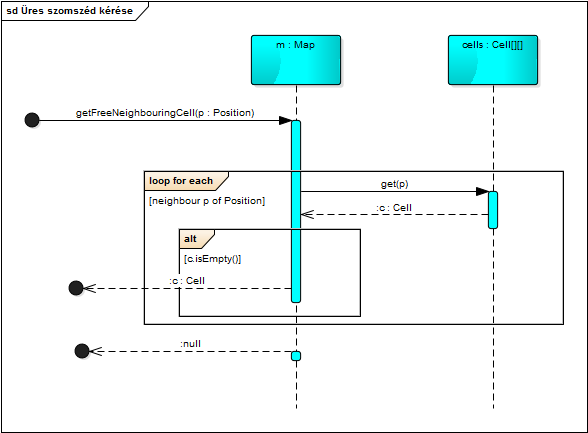
\includegraphics[width=166mm, center]{./vegleges_statikus_seq/free.png}
		\caption{Üres szomszéd keresése}
	\end{center}
\end{figure}

\begin{figure}[!htbp]
	\begin{center}
		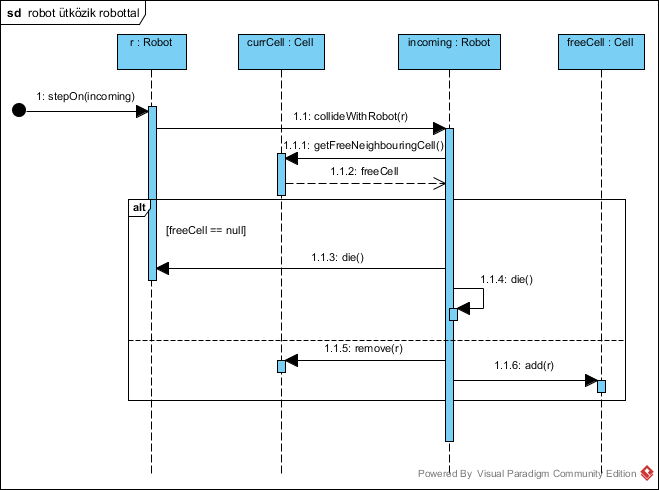
\includegraphics[width=166mm, center]{./vegleges_statikus_seq/robot_collide_robot.png}
		\caption{A robot ütközik}
	\end{center}
\end{figure}



\section{State-chartok}


\begin{figure}[h]
\begin{center}
%\includegraphics[width=17cm]{chapters/chapter04/example.pdf}
%\caption{x}
\label{fig:example3}
\end{center}
\end{figure}

